\chapter{Applied technologies} \label{related_works}

\section{Robot Operating System}

The ROS2 \cite{ROS2} (Robot Operating System 2) is not an operating system despite its name; it is a comprehensive framework for building robotic systems. This framework facilitates the development, deployment, and management of complex robotic applications by providing a collection of tools, libraries, and conventions designed to simplify the process.

At the core of ROS2 are executable units known as \textit{Nodes}. Each node is responsible for a specific task, such as sensor data processing, actuation, or decision-making. Nodes communicate with each other using a publish-subscribe messaging system, where messages are exchanged over channels called \textit{Topics}. This decoupled communication model allows for modular and flexible system design, enabling developers to easily add, remove, or modify nodes without affecting the entire system.

In addition to topics, ROS2 supports \textit{Services} and \textit{Actions}. Services provide a synchronous client-server communication model where a client sends a request to a server and waits for a response. This is useful for operations that require an immediate result, such as querying the state of a sensor or initiating a simple action.

Actions, on the other hand, are designed for long-running tasks. They allow a client to send a goal to an action server, which then executes the task and provides periodic feedback on its progress. This feedback mechanism is particularly useful for navigation tasks, where continuous updates on the robot's position, orientation, and status are essential. An action comprises a client node, a server node, a goal, and result services, along with a feedback topic, making it suitable for tasks that require continuous monitoring and dynamic adjustments.

One of the most compelling advantages of ROS2 is its language-agnostic design. Nodes can be written in multiple programming languages, primarily C++ and Python, and they can interoperate seamlessly. This interoperability is ensured by the strict message type definitions for topics, services, and actions, which remain consistent across different languages. This feature allows developers to leverage the strengths of each language; for instance, C++ for performance-critical tasks and Python for rapid prototyping and development.

In our research, we leverage ROS2 to integrate and manage the various components of our robotic system, including sensor integration, real-time mapping, and navigation. The modularity and flexibility provided by ROS2 enable us to experiment with different approaches and quickly adapt to new requirements or challenges that arise during the development process.

\section{Turtlebot4}
At Nokia, we worked on a Turtlebot4\footnote{\url{https://clearpathrobotics.com/turtlebot-4/}} which consists of an iRobot Create3 base\footnote{\url{https://edu.irobot.com/what-we-offer/create3}}, a Raspberry Pi 4 host computer, and a companion laptop attached to it. Create3 is a robot vacuum cleaner's base made for educational use. It contains the differential drive, the IR proximity sensors in the front and the docking station for charging. All in all it can be used to build more complex mobile robots.
A stereo camera and a rotating horizontal LIDAR are connected to the host computer via USB and the robot is connected to the notebook via Gigabit Ethernet so they can communicate on ROS topics. A diagram of the mentioned structure can be examined on Figure \ref{fig:mobile_robot_architecture}. The Turtlebot4 comes in two editions depending on equipment, we have the standard version. An image of the two editions of the robot can be seen on Figure \ref{fig:turtlebot4}.

\begin{figure}[htbp]
    \centering
    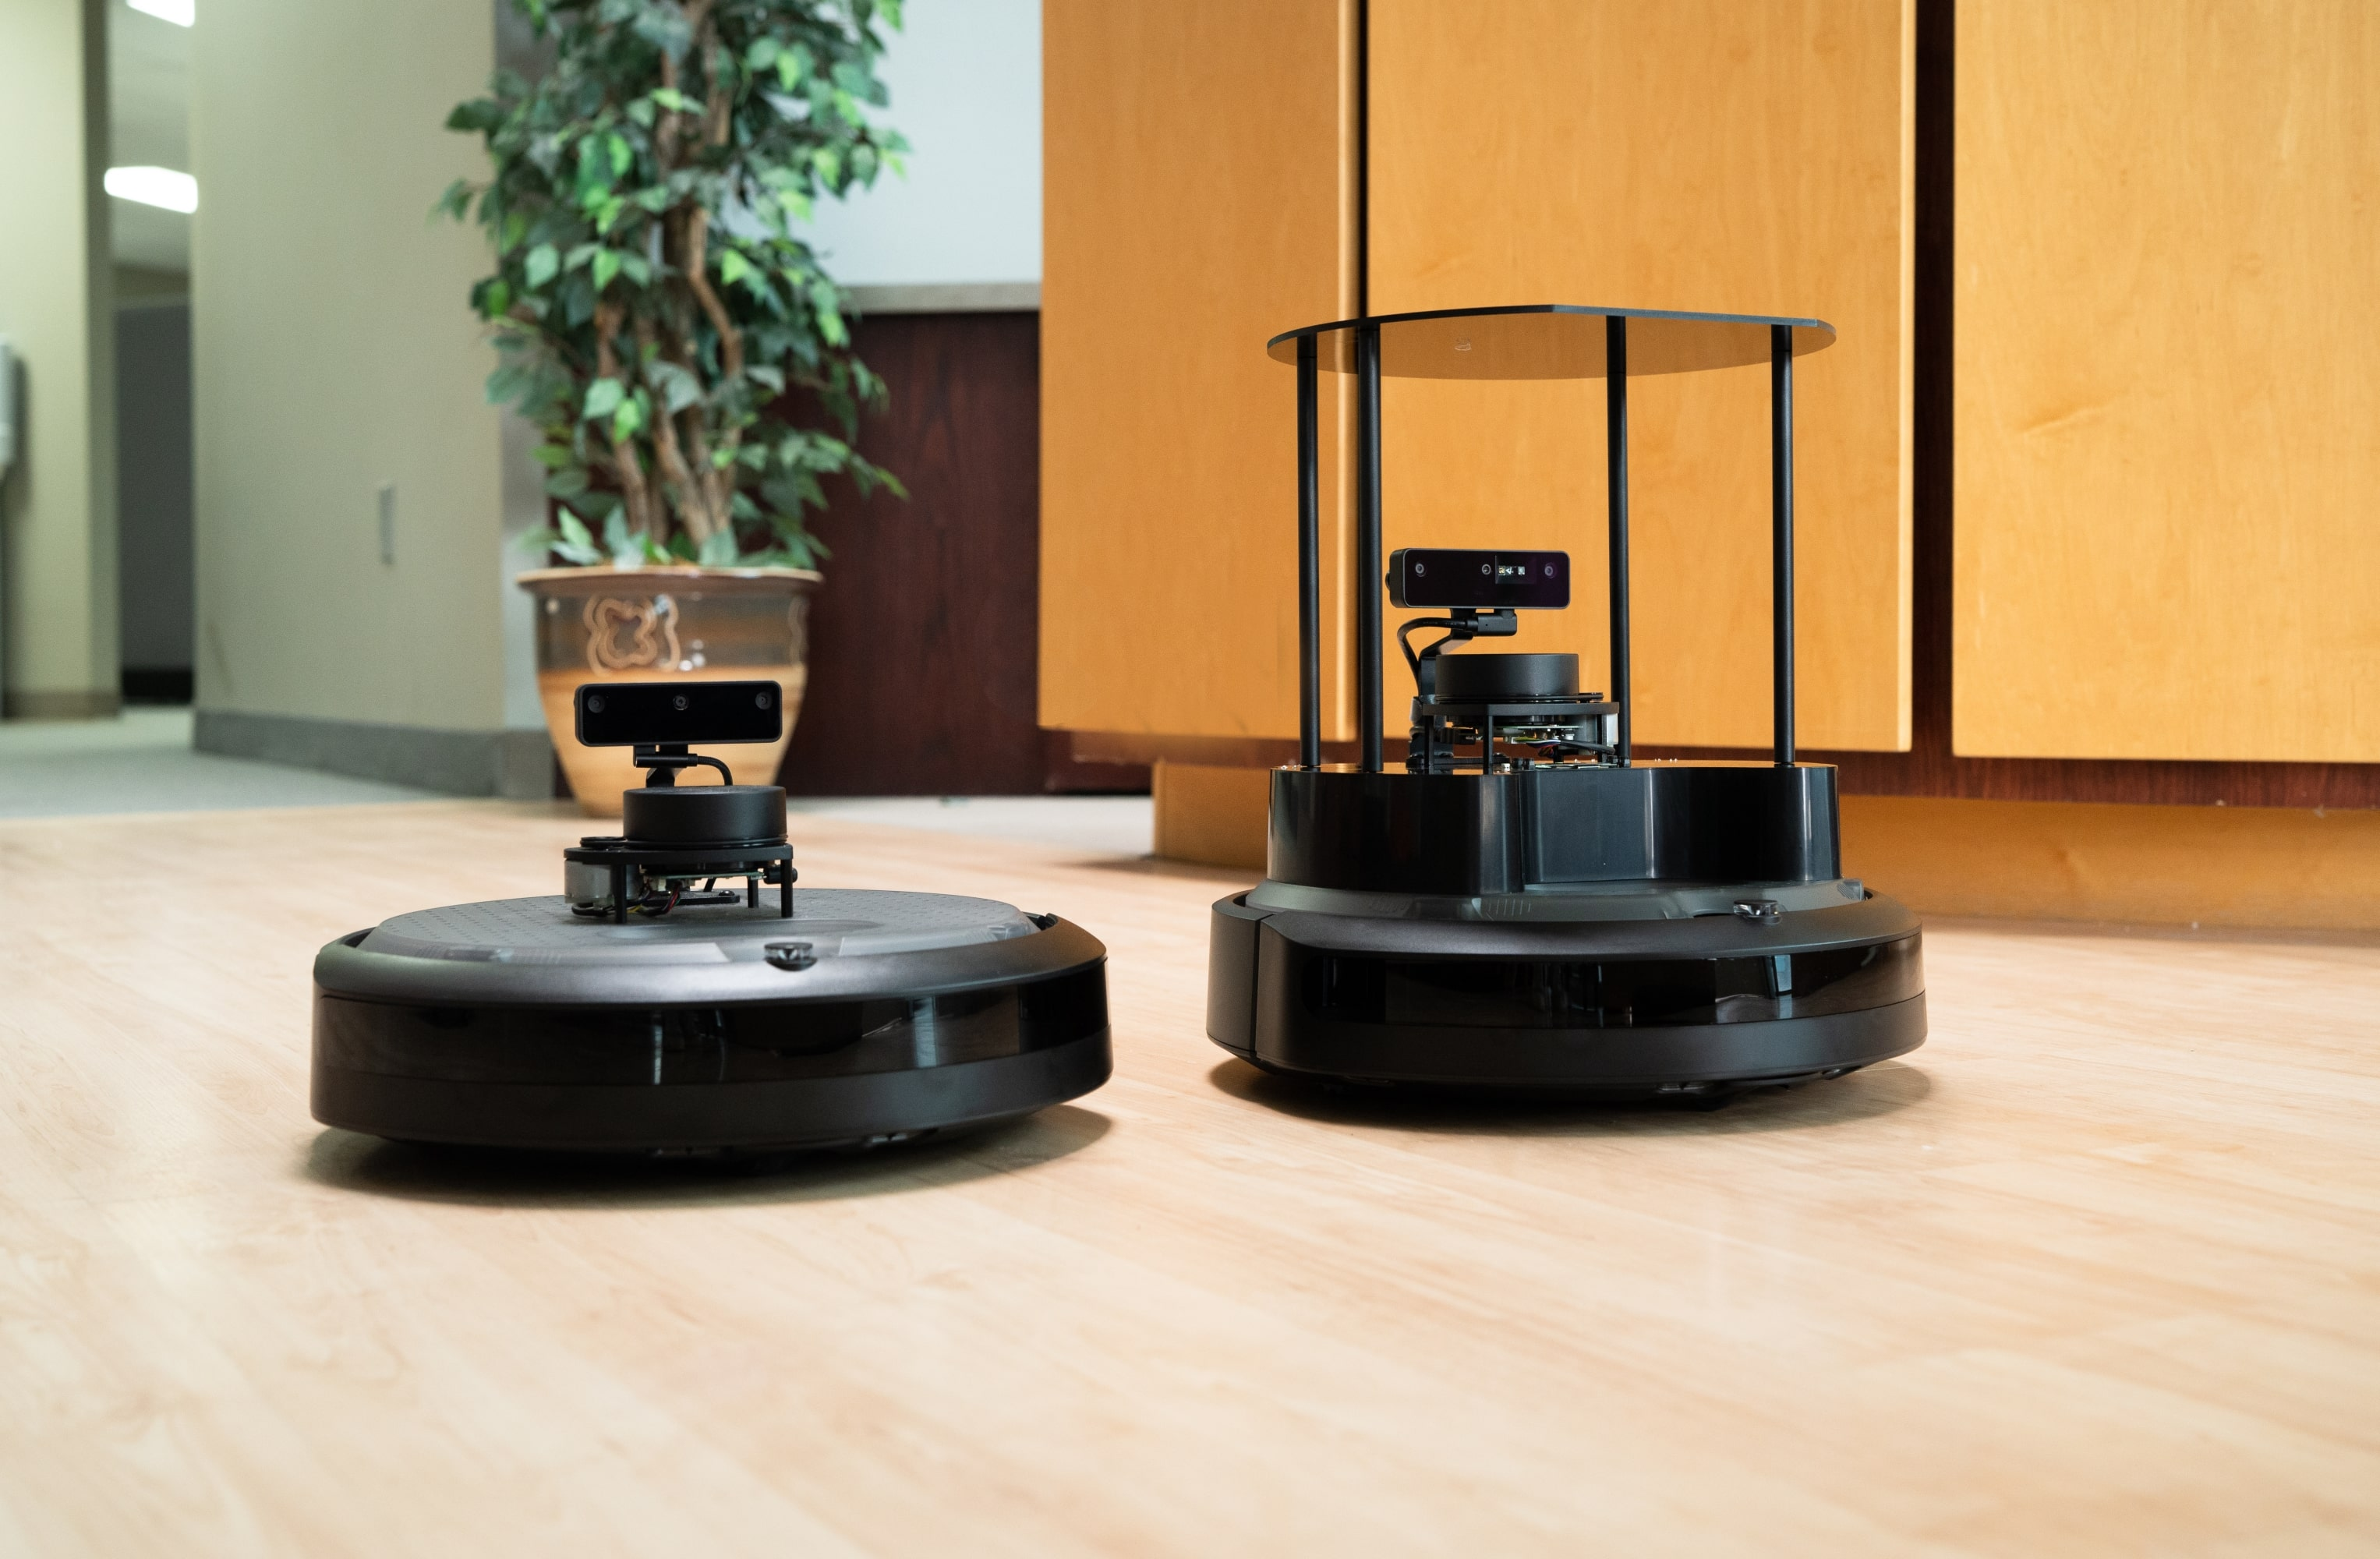
\includegraphics[width=150mm, keepaspectratio]{figures/TurtleBot4.jpg}
    \caption{Turtlebot4 Lite (left) and Turtlebot4 (source:\cite{Turtlebot4Pic})}
    \label{fig:turtlebot4}
\end{figure}

\begin{figure}[htbp]
    \centering
    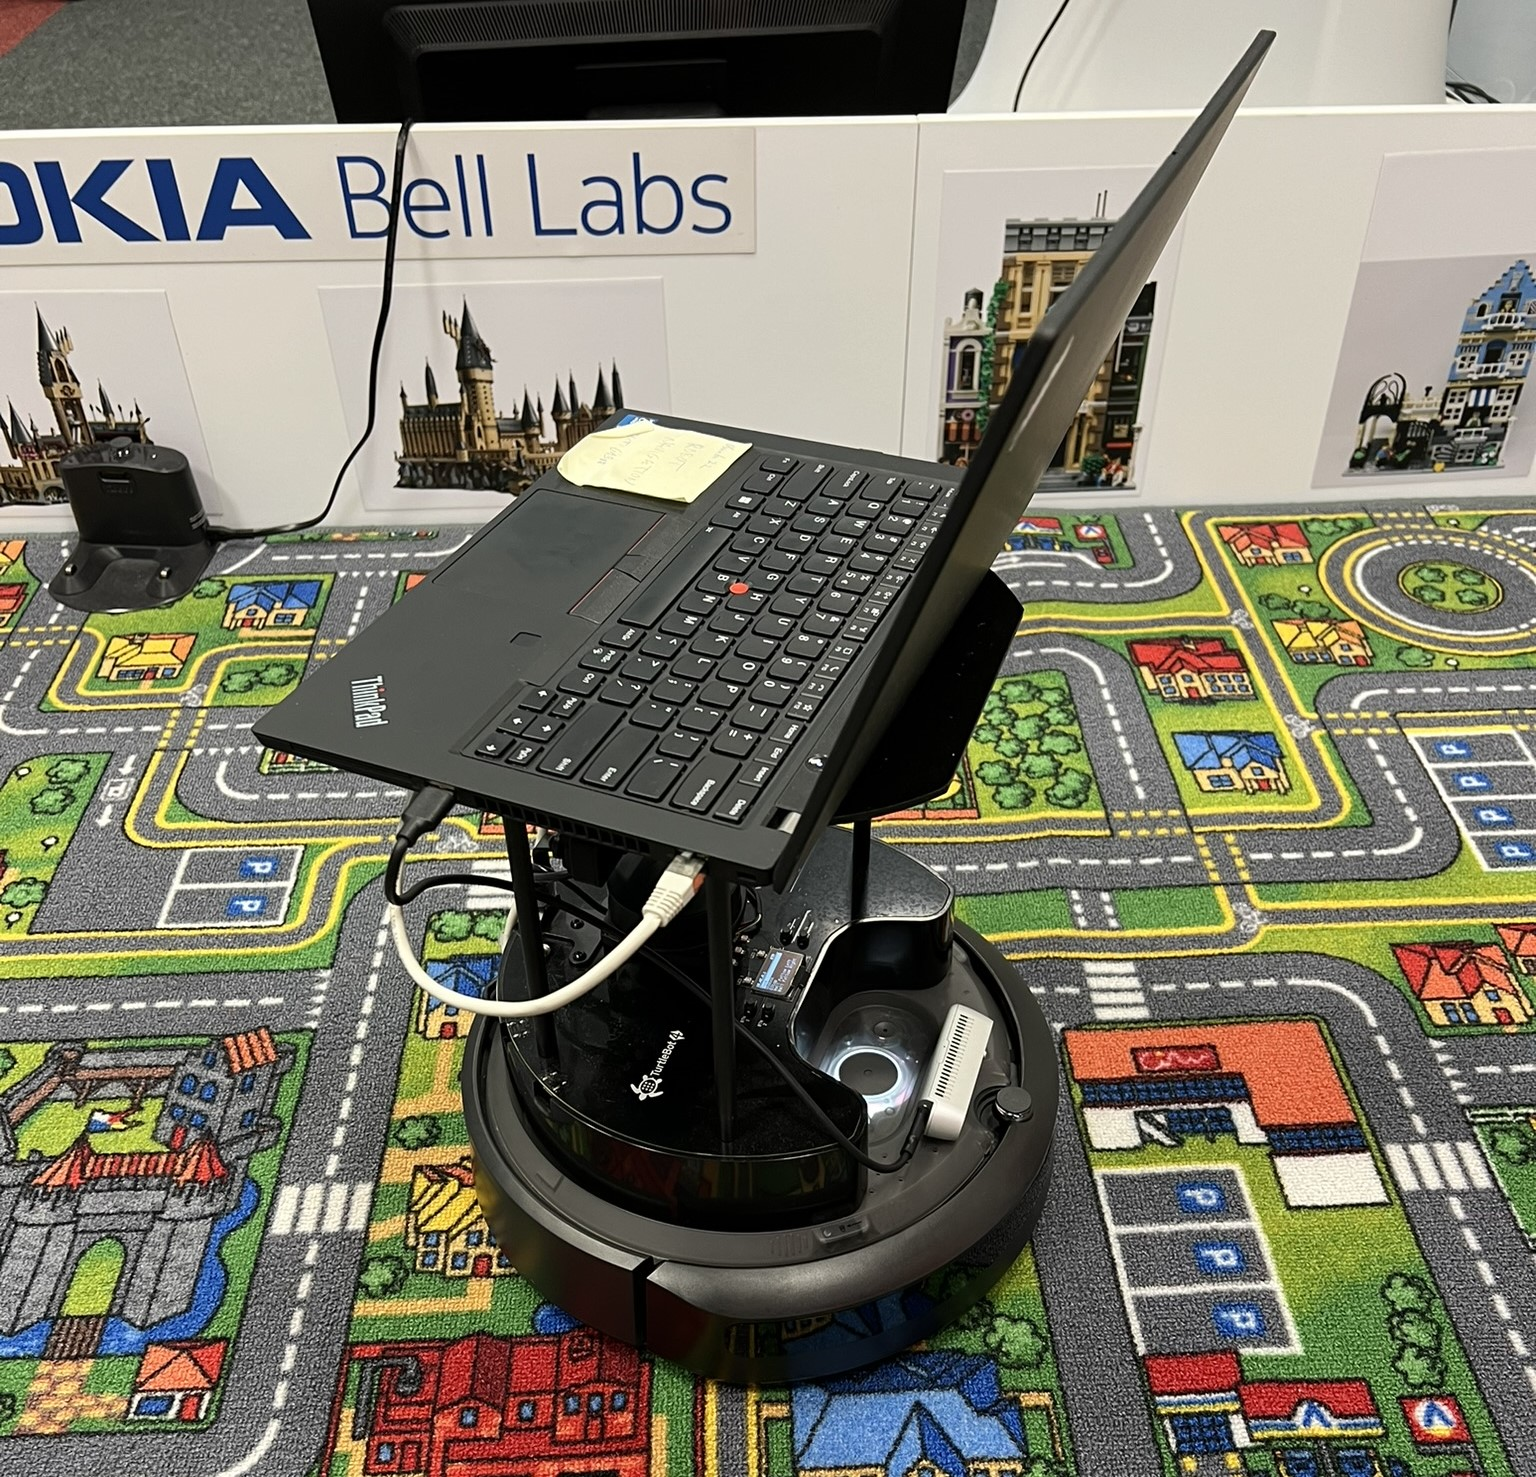
\includegraphics[width=150mm, keepaspectratio]{figures/turtlebot4_nokia.JPEG}
    \caption{Turtlebot4 at Nokia Bell Labs}
    \label{fig:turtlebot4_nokia}
\end{figure}




%\subsection{Raspberry Pi 4}
The host computer of the robot, a Raspberry Pi 4\footnote{\url{https://www.raspberrypi.com/products/raspberry-pi-4-model-b/}} is a mini PC which can be used in various applications:
at home as a desktop PC,
as a NAS (Network-Attached Storage),
as a media server,
in complex embedded systems,
in mobile robots, just to name only a few examples.
The RPi4 is equipped with a quad core ARM v8 Cortex-A72\footnote{\url{https://www.arm.com/products/silicon-ip-cpu/cortex-a/cortex-a72}} 64-bit SoC, Gigabit ethernet, 2 micro-HDMI ports which support resolution up to 4K, an USB-C power input and 2, 4 or 8 GB of RAM (it can be chosen by our needs or budget). In the Turtlebot4 the Raspberry Pi is used to run ROS2.


%\subsection{RPLIDAR-A1}
The Turtlebot4 is equipped with an RPLIDAR-A1\footnote{\url{https://www.slamtec.ai/product/slamtec-rplidar-a1/}} by Slamtech. It is a 2D LIDAR which can scan its surroundings up to 12 meters in 360°. Its maximum resolution is 1° with a maximum sampling frequency of 1\,Hz.
The sensor is plug-and-play, it has a USB interface, open-source SDK and ROS2 integration. It goes without saying, but it is worth noting that it meets the Class 1 laser safety standard and is completely safe for human eyes~\cite{LaserSafety}.

%\subsection{OAK-D Pro}
The Turtlebot 4 Standard also comes with an OAK-D Pro stereo camera as seen on Figure~\ref{fig:oak_d_pro_nokia}. OAK\footnote{\url{https://shop.luxonis.com/collections/oak-cameras-1}} is a robotic vision camera series made by Luxonis\footnote{\url{https://www.luxonis.com/}}. Additionally, I got another OAK-D model from Nokia to test my implementations at home during the semester.

The specifications of the OAK-D:
\begin{table}[h!]
\centering
\begin{tabular}{|>{\raggedright\arraybackslash}p{0.45\linewidth}|>{\raggedright\arraybackslash}p{0.45\linewidth}|}
\hline
\textbf{OAK-D} & \textbf{OAK-D Pro} \\
\hline
\begin{itemize}
    \setlength\itemsep{0em}
    \item it has an IMX378 color camera,
    \item a pair of OV9282 as the stereo cameras (grayscale),
    \item an integrated 9-axis IMU,
    \item a VPU that can run neural network models.
\end{itemize} &
\begin{itemize}
    \setlength\itemsep{0em}
    \item it has an IMX378 Auto-Focus color camera,
    \item a pair of OV9282 as stereo cameras (greyscale),
    \item it contains the VPU and the IMU as well,
    \item it supports active stereo,
    \item it has IR illumination for night vision.
\end{itemize} \\
\hline
\end{tabular}
\caption{Specifications of OAK-D and OAK-D Pro}
\end{table}


\begin{figure}[htbp]
    \centering
    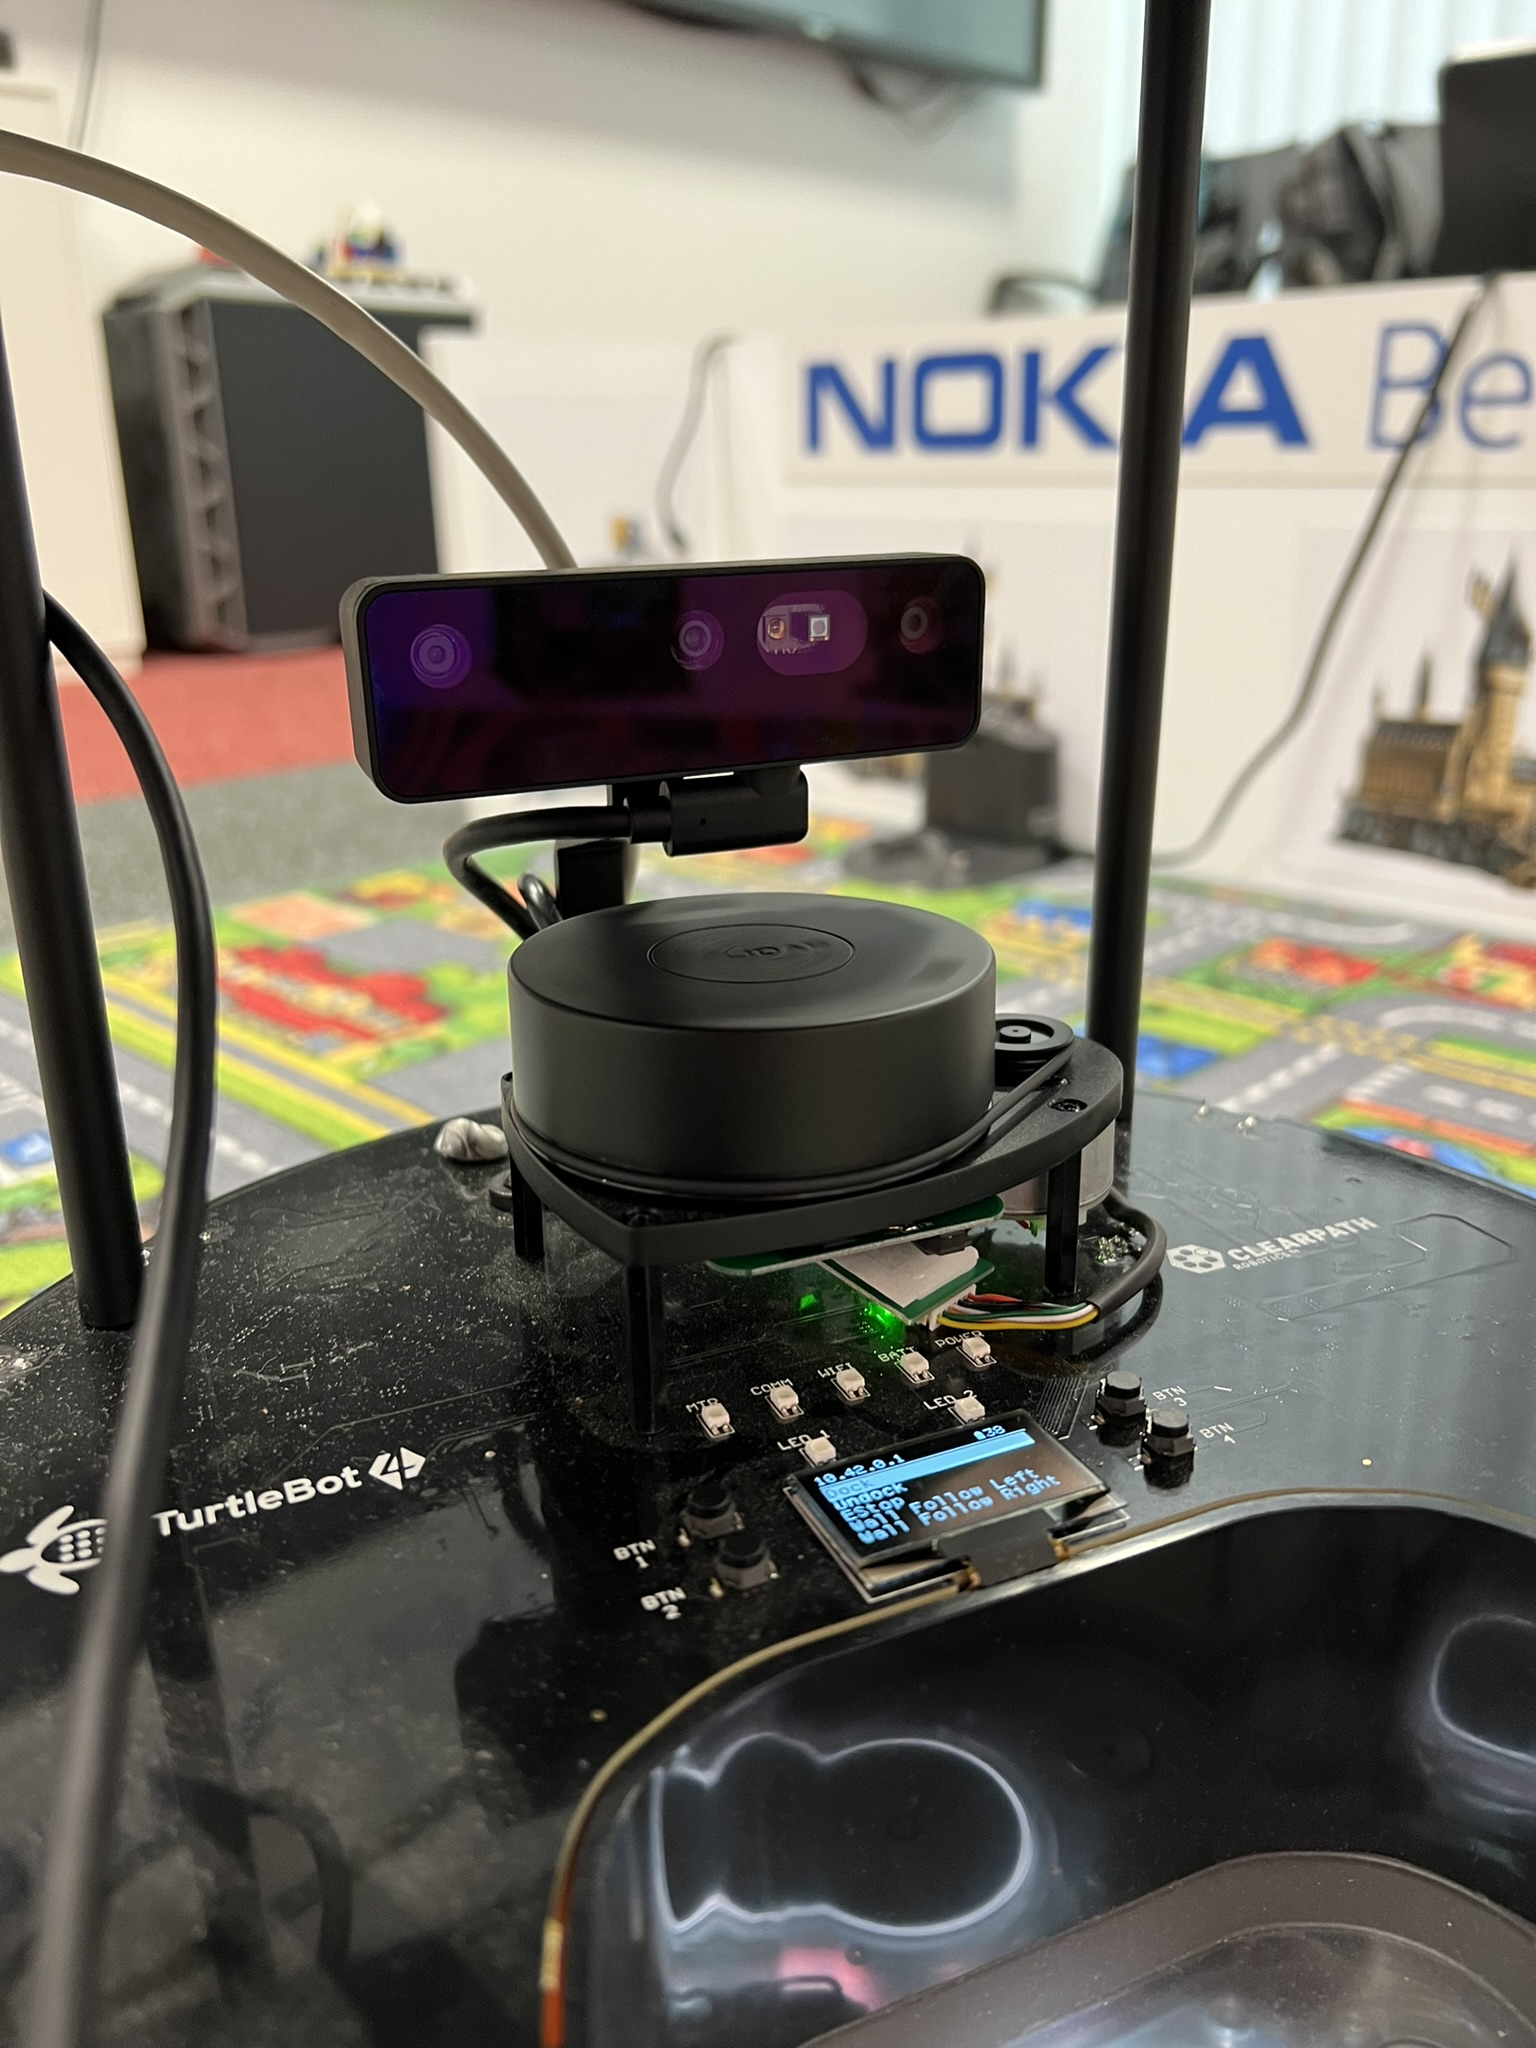
\includegraphics[width=100mm, keepaspectratio]{figures/oak_d_pro_nokia.JPEG}
    \caption{OAK-D Pro on a Turtlebot4 at Nokia Bell Labs}
    \label{fig:oak_d_pro_nokia}
\end{figure}

There are passive and active stereo cameras.
Passive stereo means the disparity between two cameras to calculate the distances between the camera and the scene points. By back-projecting a depth map into the scene, we can create a 3D point cloud of our surroundings. This method works best in environments with diverse textured surfaces because the stereo matching algorithm can only calculate the disparity values if the two cameras can see and identify corresponding points on their images. In case we point the camera to a textureless surface (for example a clean white wall) it will not be able to calculate the distances due to the lack of matching points. 
Active stereo cameras project an infrared light pattern into the scene, so they are able to find matching points even on textureless surfaces. The difference between the two methods can be observed on Figure~\ref{fig:active-passive-stereo}.

\begin{figure}[htbp]
    \centering
    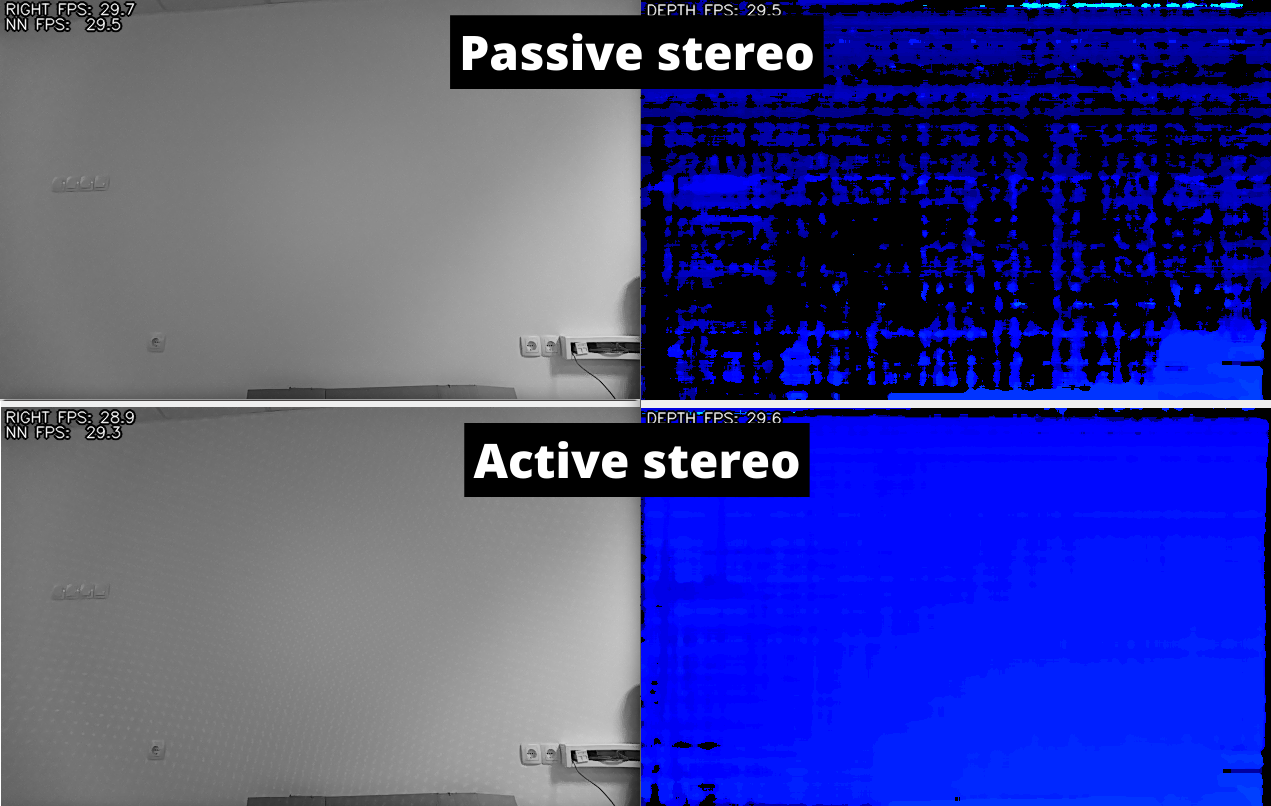
\includegraphics[width=100mm, keepaspectratio]{figures/active-vs-passive-stereo.png}
    \caption{Passive vs active stereo feature matching (source:\cite{ActivePassiveStereo})}
    \label{fig:active-passive-stereo}
\end{figure}

\begin{figure}[htbp]
    \centering
    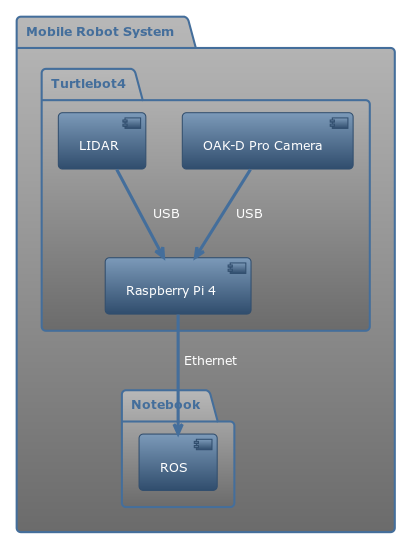
\includegraphics[width=50mm, keepaspectratio]{figures/turtlebot4_architecture.png}
    \caption{Architectural diagram of the mobile robot system at Nokia Bell Labs}
    \label{fig:mobile_robot_architecture}
\end{figure}

\FloatBarrier
\section{Spectacular AI SDK}

Spectacular AI\footnote{\url{https://www.spectacularai.com/}} is a Finnish company specialized on spatial visual-inertial motion tracking and 3D mapping. They provide an SDK\footnote{\url{https://github.com/SpectacularAI/sdk}} that can be used for various applications:
% Ensure no floats before the list
\FloatBarrier
\begin{itemize}
\setlength\itemsep{0em}
    \item pose tracking using camera and IMU fusion,
    %\item camera image visualization,
    %\item IMU localization visualization,
    \item point cloud mapping,
    \item 3D visualization of the agent trajectory
    \item AR mapping with meshes or point clouds,
    \item mapping with ROS2 visualization.
\end{itemize}
% Ensure no floats within the list
\FloatBarrier
The main goal of the SDK is to lend us a hand when we want to do SLAM with an OAK camera. It supports working with ROS through some basic ROS nodes and bridges. The SDK's main strenght is the usage of the IMU and VPU in the OAK camera.

Spectacular AI's SDK serves as a catalyst for innovation in computer vision applications, catering to a diverse range of industries and use cases. Its intuitive interface and comprehensive feature set make it a valuable tool for developers seeking to harness the full potential of OAK cameras in their projects.

\section{Neural reconstruction}

One of the various methods for neural reconstruction is Gaussian splatting~\cite{3DGS}. It is a rendering technique that offers a unique approach to representing and visualizing three-dimensional scenes. Instead of relying on traditional surface or line primitives to render objects, Gaussian splatting employs "splats", which are essentially two-dimensional discs with Gaussian distribution characteristics. These splats are strategically placed within the scene based on key points extracted from images. By overlapping these splats, the technique reconstructs the underlying geometry and appearance of the scene.

One of the primary advantages of Gaussian splatting lies in its ability to faithfully capture the intricacies of complex scenes without requiring an explicit representation of geometry. This makes it particularly useful in scenarios where the scene's geometry is challenging to model or where the available data is sparse or noisy. By leveraging the information from multiple viewpoints, Gaussian splatting can generate detailed and coherent renderings, even from limited input data.

Recent advancements in the field, particularly in the realm of Neural Radiance Fields~\cite{nerf} (NeRFs), have propelled the development of photorealistic reconstruction techniques to new heights. NeRFs, which are neural network-based models capable of synthesizing novel views of a scene from a sparse set of input images, have demonstrated remarkable success in generating high-fidelity renderings. By using NeRFs, researchers have been able to achieve even more impressive results, enabling the generation of photorealistic renderings with enhanced efficiency and accuracy.

Gaussian splatting and NeRFs opens up exciting possibilities for various applications, including virtual reality, augmented reality, computer graphics, and beyond. As research in this area continues to evolve, we can expect further innovations that push the boundaries of what is possible in three-dimensional scene reconstruction and rendering.

Our optional goal was to create photorealistic 3D models of the robot's environment from the images taken when mapping. This could be achieved with the help of Gaussian splatting. The result could be an environment's 3D model where we can place the robot's 3D model too and visualize its position real-time while it runs in localization mode using the discovered map.

\section{RTAB-Map}

RTAB-Map (Real-Time Appearance-Based Mapping~\cite{RTAB_Map_docs}) is a graph-based SLAM (Simultaneous Localization and Mapping) approach designed for long-term and large-scale mapping in real-time. It is widely used in robotics applications due to its capability to create detailed and accurate maps while efficiently managing computational resources.

RTAB-Map was introduced by Labbé and Michaud in 2013 as a solution to address the challenges of real-time 3D mapping. The core concept of RTAB-Map is to utilize an appearance-based loop closure detection method, which significantly enhances the robustness and accuracy of the mapping process. This method allows the system to recognize previously visited locations, thereby correcting the trajectory and reducing cumulative errors typically associated with SLAM algorithms.

One of the key features of RTAB-Map is its ability to handle large-scale environments. It achieves this by organizing the map into a graph structure where nodes represent keyframes, and edges represent spatial constraints between them. This graph structure is continuously optimized to improve the accuracy of the map and the estimated trajectory. Additionally, RTAB-Map employs a memory management strategy to keep the computational load manageable, ensuring that the system can operate in real-time even with extensive data.

RTAB-Map is highly versatile and supports various sensor configurations, including RGB-D cameras, stereo cameras, and LIDAR sensors. This flexibility makes it suitable for a wide range of applications, from indoor navigation to outdoor exploration. Moreover, RTAB-Map is integrated with ROS, providing a comprehensive suite of tools for robotic development and deployment.

% Do we even need this section?
\section{Localization}

After creating a detailed map, it becomes essential to explore various approaches for photorealistic localization. Photorealistic localization involves using high-fidelity 3D reconstructions of the environment to accurately determine the robot's position and orientation. This can be particularly beneficial for tasks requiring high precision, such as navigation in complex or dynamic environments.

One promising approach is to train Neural Radiance Fields (NeRFs) or create Gaussian Splats from the mapped environment. NeRFs leverage neural networks to synthesize novel views of a scene based on a sparse set of input images, providing a continuous 3D representation. Gaussian Splats, on the other hand, use point-based rendering techniques to represent the scene with a collection of Gaussian functions, enabling efficient and scalable visualization.
